\chapter{Implementation: Designing CCP Datapaths}
\label{sec:impl}
A CCP compatible datapath needs to accurately enforce the congestion control algorithm sent down by the CCP userspace module. Algorithm developers need not worry about datapath specific concerns, such as accurately measuring signals and setting the correct sending rate. Furthermore, once a datapath correctly implements support for CCP, this automatically enables support for all CCP algorithms.

In order to implement support for CCP in both QUIC and the Linux kernel, we designed a library, \ct{libccp}, to make the life of the datapath developer easier. \ct{libccp} clearly defines the requirements for a CCP datapath as well as handles CCP specific computation common to all datapaths.
We briefly discuss the CCP user-space algorithm interface, and then we describe the implementation of \ct{libccp} and how we use \ct{libccp} to design a CCP datapath in QUIC.

\section{CCP Algorithm Interface}
\label{sec:impl:alg_interface}
In the Linux kernel, congestion control decisions are tied to the ACK clock - algorithm computation is typically invoked everytime a packet ackowledgement arrives in  the networking stack.
QUIC provides an additional callback for algorithm functionality when packets are sent.
This restricts algorithm computation time to the interarrival time of ACKs or intersend time of packets; congestion control algorithms with complex computation may not perform well at high rates.
CCP, in contrast, provides both in-datapath control functionality and \textit{asynchronous} control functionality.
CCP requires algorithms to be split into two separate components explicitly: a program to execute in an off-datapath \textit{CCP agent} and a separate program to execute within the datapath itself.
Because a portion of the congestion control algorithm is now run off the datapath, the datapath must \textit{summarize} congestion signal information somehow and send it to the CCP agent.
At user specified intervals, the datapath reports congestion signal information to the CCP agent; the CCP agent can use these measurements to perform rate control decisions \textit{asynchronously} from the datapath.

The CCP API is currently written in Rust, with bindings in Python.
Users must write two functions that contain algorithm functionality to be run outside of the datapath:
  \begin{itemize}
    \item \texttt{onCreate} - Establishes algorithm state when a flow is created. Users must install some datapath program here, or else they will not get any measurements from the datapath to perform computation.
    \item \texttt{onReport} - Callback when the datapath sends a \textit{report} back to the CCP agent. This may involve some more complicated calculation that requires special user-space libraries, such as FFTs or neural networks.
  \end{itemize}

\subsection{Datapath programs}
Datapath programs are written in a simple, event driven, domain specific language.
These programs exist to provide an in-datapath, per-ACK execution environment for congestion control algorithms to update state variables per ACK and perform \textit{control actions}, in response to conditions triggered by thes variables.
Figure~\ref{fig:ccp-bbr-code} shows a CCP BBR program, that implements BBR's probe bandwidth phase.
The first block of the program defines custom variables for the user to measure; variables within the \ct{Report} block are sent back to the CCP agent on reports.
The volatile marker specifies these variables should be reset to their original values after each report.
This is followed by a series of conditions, each with a set of instructions to execute if the condition evaluates to true.

The very first condition, \ct{when true}, specifies that the block beneath should be executed everytime the program is done; here, datapath programs typically contain \textit{fold functions}.
\textit{Fold functions} are custom summaries over primitive congestion signals.
Datapath programs have read access to various \textit{primitive congestion signals}, exposed by the datapath and updated per ACK.
Table~\ref{tab:api} lists the set of congestion signals the CCP API specifies for datapaths to provide.
The BBR program uses the RTT estimate for the flow to keep track of the minimum RTT.
It also estimates the bottleneck rate of the link as the minimum of the measured receive rate and send rate.

Programs can also define conditions based on variable values and perform control actions, such as updating the sending rate, or sending a report up to the CCP agent, in response.
The following three blocks show the BBR sending pattern: it probes for the link rate by setting the rate to be 1.25x the current rate after 1 RTT.
To drain a queue that may have been create, it then sets the rate to be 0.75x the rate after one more RTT, and then it finally sets the rate as the bottleneck rate estimate after 8 RTTs.
The BBR also sends a report to the datapath after 1, 2 and 8 RTT's have passed.
Section~\ref{sec:performance:single_flow:bbr} shows results for our BBR implementation in CCP.
%{\footnotesize
%\newenvironment{code}{\captionsetup{type=listing}}{}
%\SetupFloatingEnvironment{listing}{name=Code Listing}
\begin{figure}[t!]
\begin{minted}
[
frame=lines,
framesep=2mm,
baselinestretch=1.2,
fontsize=\footnotesize,
linenos
]
{lisp}
(def
	(Report)
		(volatile minrtt +infinity)
		(volatile rate 0) 
		(pulseState 0)
	)
	(cwndCap {})
	(bottleRate {})
	(threeFourthsRate {})
    (fiveFourthsRate {})
)
(when true
	(:= Report.minrtt (min Report.minrtt Flow.rtt_sample_us))
	(:= Report.pulseState pulseState)
	(:= Report.rate (max Report.rate (min Flow.rate_outgoing Flow.rate_incoming)))
	(fallthrough)
)
(when (&& (> Micros Report.minrtt) (== pulseState 0))
	(:= Rate threeFourthsRate)
	(:= pulseState 1)
	(report)
)
(when (&& (> Micros (* Report.minrtt 2)) (== pulseState 1))
	(:= Rate bottleRate)
	(:= pulseState 2)
	(report)
)
(when (&& (> Micros (* Report.minrtt 8)) (== pulseState 2))
	(:= pulseState 0)
	(:= Cwnd cwndCap)
	(:= Rate fiveFourthsRate)
	(:= Micros 0)
	(report)
) 
\end{minted}
%\begingroup
\caption{CCP BBR datapath program that implements BBR's probe bandwidth phase.}
%\endgroup
\label{fig:ccp-bbr-code}
\end{figure}
\begin{table}
    \label{tab:api}
    \centering
    \begin{tabular}{p{0.35\columnwidth}p{0.5\columnwidth}}
        \hline
        \hline
        \multicolumn{2}{c}{Primitive congestion signals} \\
        \hline
        \hline
        \textbf{Signal} & \textbf{Definition} \\
        \texttt{Ack.bytes\_acked}, \texttt{Ack.packets\_acked} & In-order acknowledged \\
        \texttt{Ack.bytes\_misordered}, \texttt{Ack.packets\_misordered} & Out-of-order acknowledged \\
        \texttt{Ack.ecn\_bytes}, \texttt{Ack.ecn\_packets} & ECN-marked \\
        \texttt{Ack.lost\_pkts\_sample} & Number of lost packets \\
        \texttt{Ack.now} & Datapath time (e.g., wall clock time)\\
        \texttt{Flow.was\_timeout} & Did a timeout occur? \\
        \texttt{Flow.rtt\_sample\_us} & A recent sample RTT \\
        \texttt{Flow.rate\_outgoing} & Outgoing sending rate \\
        \texttt{Flow.rate\_incoming} & Receiver-side receiving rate  \\
        \texttt{Flow.bytes\_in\_flight}, \texttt{Flow.packets\_in\_flight} & Sent but not yet acknowledged \\
        & \\
        \hline
        \hline
        \multicolumn{2}{c}{Operators} \\
        \hline
        \hline
        \textbf{Class} & \textbf{Operations} \\
        Arithmetic & $+, -, *,$~/$,$ EWMA \\
        Assignment & $:=$ \\
        Comparison & $==, <, >$, or, and \\
        Conditionals & If (branching) \\
        & \\
        \hline
        \hline
        \multicolumn{2}{c}{Variable Scopes} \\
        \hline
        \hline
        \textbf{Scope} & \textbf{Description} \\
        \texttt{Ack} & Signals measured per packet \\
        \texttt{Flow} & Signals measured per connection \\
        \texttt{Timer} & Multi-resolution timer that can be zeroed by a call to \texttt{reset} \\
    \end{tabular}
    %\vspace{0.075in}
    \caption{Fast path language: primitive signals, operators, and scopes. As per the CCP API, datapaths must exposes these signals and operators}
\end{table}


\section{Responsibilities of a CCP Datapath}
\label{sec:impl:datapath_responsibilites}
A CCP datapath has four main responsibilities.
  \begin{itemize}
    \item Establish an IPC mechanism.
    \item Enforce congestion windows and pacing rates.
    \item Update the congestions signals listed in Table~\ref{tab:api} as ACKs are received.
	\item Parse and serialize the datapath program sent by the CCP agent, and execute the datapath program every ACK. This may cause the datapath to send a report up to the CCP agent.
  \end{itemize}
First, it must communicate with the CCP agent using some interprocess communication (IPC) mechanism.
The current implementation of the CCP agent expects that the datapath communicates through a single persistent connection.
Regardless of how many new flows enter, the datapath must be able to send and receive messages about all flows over this single connection.
It must assign flow IDs and uses these IDs to distinguish between flows when serializing and deserializing messages.\par

In order to accurately enforce the sending patterns of the congestion control algorithm, datapaths should enforce pacing rates and congestion windows separately. This would allow an algorithm to specify a congestion window with a rate cap, in order to prevent bursty transmission.
The datapath must install and execute the programs sent down by the CCP agent, which specify how to aggregate and report measurements over the congestion primitives, how to set the congestion window and pacing rate and when to report measurements.
While the CCP agents compiles the user's programs into a serialized set of instructions for the datapath, the datapath must ensure safe execution of the instructions.
For the Linux kernel datapath, this involves ensuring that instructions cannot cause a divide by zero that would crash the kernel.
However, the domain specific language is very limited; programs may not enter loops, allocate memory, define functions or use pointers.

\section{\ct{libccp}}
\label{sec:impl:libccp}
To help add CCP support in various datapaths, we implemented a shared library in C, named \ct{libccp}, that provides a reference implementation for the features common to all CCP datapaths: serialization of messages and execution of the program sent down by the userspace agent.
As we built our kernel, QUIC and mTCP datapaths simultaneously, a shared library enabled code reuse across different implementations.
As \ct{libccp} implements much of the necessary functionality, datapath developers solely need to focus on: 
\begin{enumerate}
    \item Defining primitive congestion signals.
    \item Exposing mechanisms to set congestion windows and pacing rates.
\end{enumerate}
Specifically, to implement the datapath API, datapaths must provide a set of function pointers, set up a compatible form of IPC (character device or netlink sockets for kernel datapaths, and unix sockets for user-space datapaths), and update the congestion signal primitives as the flow runs.
Datapath developers must provide function pointers that do the following:
\begin{enumerate}
    \item Set a congestion window (in bytes)  or pacing rate (either an absolute rate, or relative to current rate) given a flow ID.
    \item Provide a notion of time: now, since, and after (in microseconds).
    \item Send a message through the IPC to the userspace CCP agent.
\end{enumerate}
Each of these functions takes in a pointer to \ct{struct ccp\_connection}, which contains state for this flow. \ct{ccp\_connection} includes one field for datapath specific state per flow. In the Linux kernel, for example, this is pointer to the \ct{tp\_sock} object, to access congestion state for the correct connection.

In return, \ct{libccp} provides two functions that the datapath can call:
\begin{itemize}
    \item \texttt{ccp\_invoke}: After updating the primitive congestion signals on ACKs and timeouts, \texttt{ccp\_invoke} will invoke the program state machine stored inside \libccp. This will run through the currently installed program, ending with an optional report to the userspace CCP agents. The program will automatically invoke the function pointers that set the rate or cwnd within the datapath.
    \item \texttt{ccp\_read\_msg}: Upon reading a message from the IPC mechanism, the datapath can call \texttt{ccp\_read\_msg}. 
        Currently, CCP can send down two types of messages: a message that updates the value of a particular variable in the datapath program (including the rate or congestion window), or a message to install a new fast path program completely. \ct{libccp} will deserialize the message to parse both the flow ID and message type from the header, in order to perform the correct update for the correct flow.
\end{itemize}

With the architecture of the \ct{libccp}, adding support into QUIC for supporting CCP was relatively easy.

\section{Current Congestion Control Architecture in QUIC}
\label{sec:impl:currentq_quic}
As discussed in Section~\ref{sec:relwork:quic}, QUIC already supports pluggable congestion control in user-space.
\begin{figure}[h]
\centering
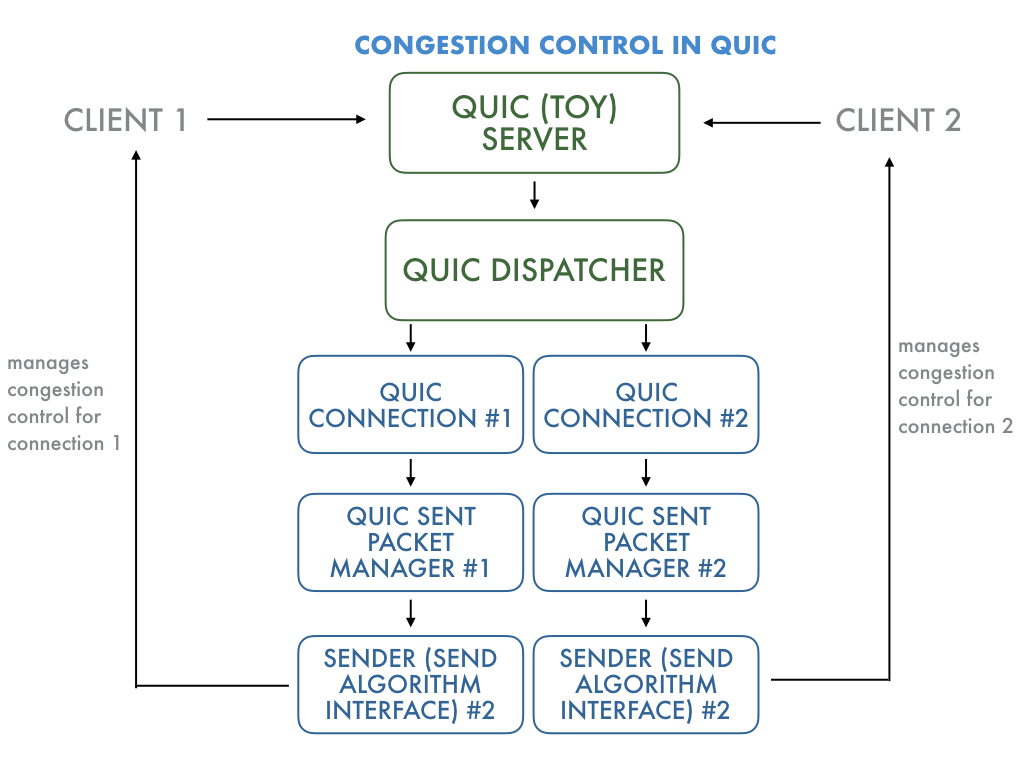
\includegraphics[scale=.45]{implementation/quiccc}
\caption{In QUIC, when the toy server sees a client request, the \ct{SimpleDispatcher} object spawns a new \ct{QuicConnection} object that handles the connection. To manage sending packets, the \ct{QuicConnection} object creates a \ct{QuicSentPacketManager}. The \ct{QuicSentPacketManager} creates a \ct{Sender} object that uses the function callbacks from the \ct{SendAlgorithmInterface} specified as the current congestion control setting.}
\label{fig:quiccc_diagram}
\end{figure}

As Fig~\ref{fig:quiccc_diagram} shows, QUIC uses the \ct{SendAlgorithmInterface} class to allow developers to add in new algorithms.
QUIC uses the \ct{GetCongestionWindow()} and \ct{PacingRate()} functions to access the congestion window and pacing rate, so senders can implement these functions to expose the rate and window they calculate.
Pacing is implemented through a separate sender class with a token bucket scheme.
When deciding whether to send more, the \ct{QuicConnection} object invokes the \ct{CanSend} callback.
This function takes in the number of bytes in flight and checks whether the congestion window is less.
If pacing is enabled and the pacing rate is not 0, the \ct{QuicConnection} checks whether sending should be delayed due to pacing.

Three functions allow senders to measure the congestion signals specified in Table~\ref{tab:api}:
\begin{itemize}
	\item \ct{OnCongestionEvent}: This callback is triggered on new ACKs and lost packets; it provides a vector of acked packets, a vector of lost packets, a boolean indicating if the RTT has been updated, and the prior in flight byte count.
	\item \ct{OnPacketSent}: This callback provides new information on the current number of bytes in flight when packets are sent.
	\item \ct{OnRetransmissionTimeout}: This callback allows senders to take any special actions in the case of timeouts; packets are not counted as lost in the case of timeouts.
\end{itemize}

The \ct{SendAlgorithmInterface} allows for congestion signal measurement and rate control within QUIC.
In order to support CCP, the datapath must also implement an IPC mechanism to communicate with the CCP agent.
Each sender object could independently spawn an IPC mechanism, such as a UDP socket, to communicate with the CCP agent.
However, the current implementation of the CCP agent expects that communication regarding all flows is multiplexed onto a single connection.
Since each sender is an independent object, it only knows about its own flow; some object higher in the hierarchy in Figure~\ref{fig:quiccc_diagram} must control IPC with the CCP agent.

\section{Integrating \ct{libccp} in QUIC}
\label{sec:impl:quic_ccp}
\subsection{Architecture}
\begin{figure}[h]
\centering
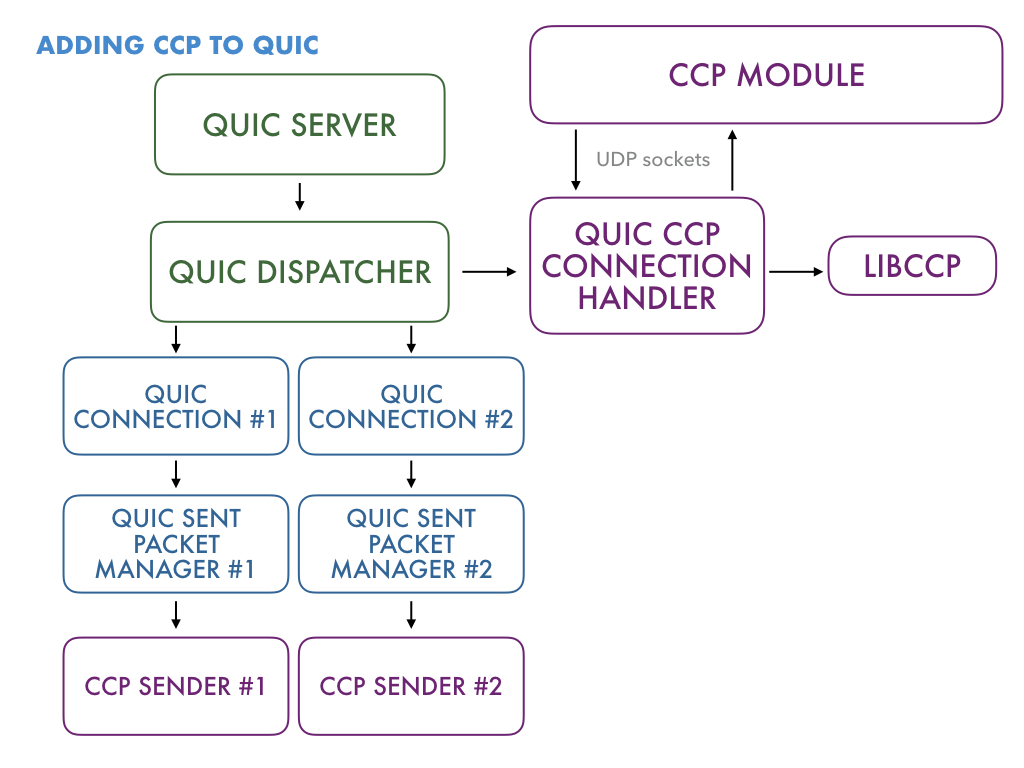
\includegraphics[scale=.45]{implementation/ccpquic_diagram}
\caption{The \ct{QuicCCPConnectionHandler} class implements the \libccp API. It provides the time related functions through the C++ standard library's wall clock time. By passing in the pointer to the specific \ct{QuicConnection} object to a call to \ct{Set\_Congestion\_Window}, the CCP connection handler propagates the instruction down to the specific CCP sender object.}
\label{fig:ccpquic_diagram}
\end{figure}


To implement CCP support in QUIC, we add a new \ct{CCPSender} class that implements the \ct{SendAlgorithmInterface}.
To handle IPC communication with the CCP Agent, we create a new object, the \ct{CCPConnectionHandler}, that sends and receives messages using UDP sockets.
In addition, the function pointers necessary for \ct{libccp}, such as the functions to set a flow's congestion window or rate, are provided through this class.
The \ct{SimpleDispatcher} owns the \ct{CCPConnectionHandler}; Figure~\ref{fig:ccpquic_diagram} details how the new classes fit into the overall QUIC congestion control architecture.
Upon starting a new connection, the connection handler sets up CCP related state for the flow.
It saves a pointer to the \ct{QuicConnection} object in the \ct{libccp} state for this flow.
Later, when the datapath program is running and it must set a window or pacing rate for this flow, it calls the set window pointer exposed by the \ct{CCPConnectionHandler} with the \ct{QuicConnection} pointer as argument.

\subsection{Congestion Signal Measurement}
\label{sec:impl:congestion_signals}
\begin{table}
    \label{tab:quicsignaldef}
    \centering
    \begin{tabular}{p{0.35\columnwidth}p{0.5\columnwidth}}
        \hline
        \hline
        \multicolumn{2}{c}{Primitive congestion signals} \\
        \hline
        \hline
        \textbf{Signal} & \textbf{Definition} \\
        \texttt{Ack.bytes\_acked}, \texttt{Ack.packets\_acked} & Number of bytes received in order in a call to \ct{OnCongestionEvent} before the first lost packet, from the \ct{AckedPackets} vector passed in as an argument \\
        \texttt{Ack.bytes\_misordered}, \texttt{Ack.packets\_misordered} & Number of bytes received in the \ct{AckedPackets} vector with a sequence number greater than the sequence number of the first lost packet. \\
        \texttt{Ack.lost\_pkts\_sample} & Number of lost packets, i.e. size of the \ct{LostPackets} passed into the \ct{OnCongestionEvent} function. \\
        \texttt{Ack.now} & C++ Standard library wall clock time\\
        \texttt{Flow.was\_timeout} & True when \ct{OnRetransmissionTimeout} is called \\
        \texttt{Flow.rtt\_sample\_us} & The most recent new RTT sample.\\
        \texttt{Flow.rate\_outgoing} & Outgoing sending rate \\
        \texttt{Flow.rate\_incoming} & Receiver-side receiving rate, measured at the sender.  \\
        \texttt{Flow.bytes\_in\_flight}, \texttt{Flow.packets\_in\_flight} & Updated whenever a packet is sent for a new estimate of the number of bytes currently in the pipe. \\
    \end{tabular}
    %\vspace{0.075in}
    \caption{On ACKs, the \ct{CCPSender} uses these definitions to update the calculations of the primitive congestion signals}
\end{table}

Each sender individually measures congestion signals and calls \ct{ccp\_invoke} to trigger execution of the fastpath program within \libccp.
Table~\ref{tab:quicsignaldef} specifies how QUIC calculates each congestion signal primitive.
As discussed in Section~\ref{sec:relwork:quic}, QUIC assigns a new sequence number for every retransmission of a packet.
QUIC, unlike TCP, provides fine grained loss information and exposes exact information about which sequence numbers are lost, within a block of packets.
QUIC currently does not support ECN, so it does not expose ECN related information.
This means it cannot support algorithms such as DCTCP~\cite{dctcp} or ABC~\cite{abc}.

\section{Summary of Implementation}
\label{sec:impl:summary}
\label{impl_summary}
We implement CCP support in the QUIC Toy Server, in the publicly released chromium code base.
The changes, in total, include:
\begin{itemize}
    \item New \ct{CCPSender} that implements the send algorithm interface
    \item Modify \ct{QuicConnection} and \ct{QuicSentPacketManager} classes to allow setting windows for the underlying \ct{CCPSender}
    \item New \ct{QuicCCPConnectionHandler} class
    \item Modify \ct{QuicSimpleDispatcher}, used by the toy server, to spawn a connection handler when starting a new connection
    \item Add \ct{libccp} as a third party library
    \item Command line options when running the toy server to control which congestion control option is set
    \item New congestion window logger class to help with experimenting
\end{itemize}
All the changes are based on top of Chromium commit hash \textbf{dedfa29047}, and consist of about 1050 new lines of code.
\ct{libccp} is about a 1000-line C library.
 
